\documentclass[xcolor=dvipsnames,table]{beamer}

\usepackage{latexsym}
\usepackage[utf8]{inputenc}
\usepackage[brazil]{babel}
\usepackage{amssymb}
\usepackage{amsmath}
\usepackage{stmaryrd}
\usepackage{fancybox}
\usepackage{datetime}
\usepackage[T1]{fontenc}
\usepackage{graphicx}
\usepackage{graphics}
\usepackage{url}
\usepackage{algorithmic}
\usepackage{algorithm}
\usepackage{acronym}
\usepackage{array}

\newtheorem{definicao}{Definio}
\newcommand{\tab}{\hspace*{2em}}

\mode<presentation>
{
  \definecolor{colortexto}{RGB}{0,0,0}
 
  \setbeamertemplate{background canvas}[vertical shading][ bottom=white!10,top=white!10]
  \setbeamercolor{normal text}{fg=colortexto} 

  \usetheme{Warsaw}
}

\title{Pontes e Trilhas} 

\author{
  Esdras Lins Bispo Jr. \\ \url{bispojr@ufg.br}
  } 
 \institute{
  Teoria de Grafos \\Bacharelado em Ciência da Computação}
\date{\textbf{21 de junho de 2016} }

\logo{
\includegraphics[width=1cm]{images/ufgJataiLogo.png}}

\begin{document}

	\begin{frame}
		\titlepage
	\end{frame}

	\AtBeginSection{
		\begin{frame}{Sumário}%[allowframebreaks]{Sumário}
    		\tableofcontents[currentsection]
    		%\tableofcontents[currentsection, hideothersubsections]
		\end{frame}
	}

	\begin{frame}{Plano de Aula}
		\tableofcontents
		%\tableofcontents[hideallsubsections]
	\end{frame}
	
	\begin{frame}{Bônus (0,5 pt)}
		\begin{block}{Desafio}
			\begin{itemize}
				\item {E 1.151} 
                \item Candidaturas até amanhã (21 de junho, 13h30); 
                \item Apresentação e resposta por escrito $\rightarrow$ \\Terça (28 de junho, 15h30); 
                \item 20 minutos de apresentação.
			\end{itemize}
		\end{block}
        \begin{block}{Referência}
			FEOFILOFF, P. {\bf Exercícios de Teoria dos Grafos}, \\
			BCC, IME-USP, 2012. 
		\end{block}	
	\end{frame}
	
	\section{Pensamento}
	\begin{frame}{Pensamento}
  		\begin{center}
    		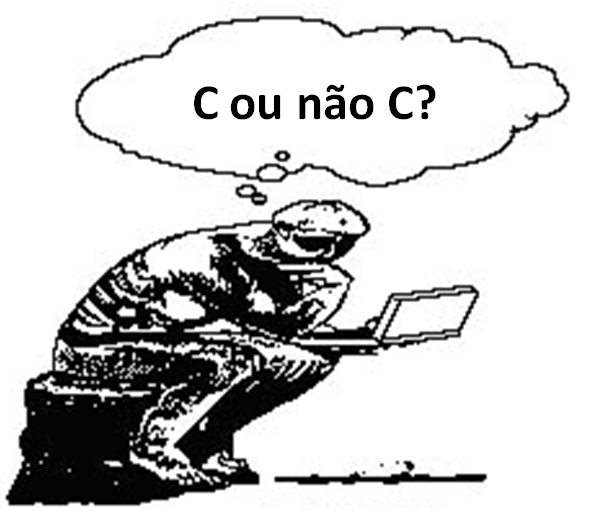
\includegraphics[width=7cm]{images/pensamento.png}
  		\end{center}
	\end{frame}
	
	\begin{frame}{Pensamento}
		\begin{columns}
			\column{.4\textwidth}  		
		  		\begin{center}
		    		
\includegraphics[height=.5\textheight]{images/desconhecido.jpg}
		  		\end{center}
			\column{.6\textwidth}  		
				\begin{block}{Frase}
					\begin{center}
						{\large A árvore quando está sendo cortada, observa com tristeza que o cabo do machado é de madeira.}
					\end{center}
				\end{block}		  		
		  		\begin{block}{Quem?}
		  			\begin{center}
						{\bf Provérbio Árabe}
					\end{center}
				\end{block}
		\end{columns}
	\end{frame}
    
    \section{Revisão}
	
	\subsection{Caminhos e circuitos em grafos}
	\begin{frame}{Caminhos e circuitos em grafos}
		\begin{block}{Caminho em um grafo}
			Se um caminho $v_1 \ldots v_p$ é subgrafo de $G$, dizemos simplesmente que $v_1 \ldots v_p$ {\bf é um} caminho em $G$ ou que \\$G$ {\bf contém} o caminho $v_1 \ldots v_p$.
		\end{block}
		\begin{exampleblock}{Circuitos em um grafo}
			Aplica-se identicamente a circuitos.
		\end{exampleblock} 
	\end{frame}
	
	\begin{frame}{Caminhos e circuitos em grafos}
		\begin{block}{Nomenclatura}
			Se $v$ e $w$ são os dois extremos de um caminho em $G$, é cômodo dizer que o caminho vai de $v$ a $w$ ou que começa em $v$ e termina em $w$.
		\end{block}
		\begin{alertblock}{Cuidado!}
			Use estas expressões com cautela pois caminhos são objetos estáticos e não têm orientação.
		\end{alertblock}
	\end{frame}
	
	\begin{frame}{Caminhos e circuitos em grafos}
		\begin{block}{Caminho máximo em $G$}
			Um caminho $P$ em um grafo $G$ é máximo se $G$ não contém um caminho de comprimento maior que o de $P$.
		\end{block}
		\begin{block}{Caminho maximal em $G$}
			Um caminho $P$ em $G$ é maximal se não existe caminho $P'$ em $G$ tal que $P \subset P'$.
		\end{block}
		\begin{block}{Caminho Hamiltoniano}
			Um caminho é {\bf hamiltoniano} se contém todos os vértices do grafo.
		\end{block}
	\end{frame}	
	
	\subsection{Cortes}
	\begin{frame}{Cortes}
		\begin{block}{Definição}
			\begin{itemize}
				\item Suponha que $X$ é um conjunto de vértices de um grafo $G$.
				\item O {\bf corte} associado a $X$ (ou {\bf franja} de $X$) é o conjunto de todas as arestas que têm uma ponta em $X$ e outra em $V_G \setminus X$.
			\end{itemize}
		\end{block}
		\begin{block}{Notação}
			O corte associado a $X$ será denotado por
			\begin{center}
				$\partial_G (X)$
			\end{center}
		\end{block} 
		\begin{alertblock}{Outros autores...}
			Alguns preferem escrever $\delta(X)$ ou $\nabla(X)$.
		\end{alertblock}
	\end{frame}
	
	\begin{frame}{Cortes}
		\begin{block}{Cortes triviais}
			\begin{itemize}
				\item $\partial( \emptyset )$; 
				\item $\partial( V_G )$.
			\end{itemize}
		\end{block} 
		\begin{block}{Corolário}
			$|\partial(\{v\})| = d(v)$
		\end{block}
		\begin{block}{Grau de um conjunto}
			\begin{itemize}
				\item Diremos que $|\partial(X)|$ é o {\bf grau} de $X$; 
				\item Denotamos este número como se segue:
					\begin{center}
						$d(X) := |\partial(X)|$
					\end{center}
			\end{itemize}
		\end{block}
	\end{frame}
	
	\begin{frame}{Cortes}
		\begin{block}{Corte - Definição}
			Um {\bf corte} ({\it = cut = coboundary}) em um grafo $G$ é qualquer conjunto da forma $\partial(X)$, em que $X$ é um subconjunto de $V_G$.
		\end{block} 
		\begin{alertblock}{Cuidado}
			Um corte é um conjunto de arestas, não de vértices.
		\end{alertblock}
	\end{frame}
	
	\section{Pontes}
	\begin{frame}{Pontes}
		\begin{block}{Definição}
			Uma {\bf ponte} ($bridge$) em um grafo $G$ é qualquer aresta $e$ tal que 
			\begin{center}
				$c(G - e) > c(G)$,  
			\end{center}
			ou seja, $G - e$ tem mais componentes que $G$.				
		\end{block} \pause
		\begin{block}{Outros nomes}
			\begin{itemize}
				\item {\bf istmo} ({\it isthmus}), ou 
			 	\item {\bf aresta de corte} ({\it cut edge}).
			 \end{itemize}
		\end{block}
	\end{frame}
	
	\begin{frame}{Pontes}
		\begin{block}{Corolário}
			Uma aresta $a$ é ponte se e somente se o conjunto $\{ a \}$ é um corte do um grafo.
		\end{block} \pause
		\begin{block}{Pontes $\times$ Circuitos}
			Em qualquer grafo, toda aresta é uma ponte ou pertence a um circuito, mas não ambos (E. 1.199).
		\end{block}
	\end{frame}
	
	\section{Trilhas}
	\begin{frame}{Trilhas}
		\begin{block}{Passeio}
	Um {\bf passeio} ({\it walk}) em um grafo é qualquer sequência finita $(v_0, v_1, v_2, \ldots, v_{k-1}, v_k)$ de vértices tal que $v_i$ é adjacente a $v_{i-1}$ para todo $i$ entre 1 e $k$.
		\end{block} \pause
		\begin{block}{Detalhe}
			Os vértices do passeio podem não ser distintos dois a dois.
		\end{block} \pause
		\begin{block}{Trilha}
			Uma {\bf trilha} ({\it trail}) é um passeio sem arestas repetidas.
		\end{block}
	\end{frame}
	
	\begin{frame}{Trilhas}
		\begin{block}{Passeio ou trilha fechados}
			\begin{itemize}
				\item Um passeio é fechado se $v_0 = v_k$;
				\item Uma trilha é fechada se $v_0 = v_k$;
			\end{itemize}			
		\end{block} \pause
		\begin{block}{Expressões comuns}
			\begin{itemize}
				\item $v_0$ é a {\bf origem} do passeio;
				\item $v_k$ é o {\bf término} do passeio;
				\item o passeio {\bf vai de} $v_0$ a $v_k$;
				\item o passeio {\bf liga} $v_0$ a $v_k$;
			\end{itemize}
		\end{block}
	\end{frame}
	
	\begin{frame}{Trilhas}
		\begin{block}{Passeio simples}
			Um passeio é {\bf simples} se os seus vértices são distintos dois a dois.
		\end{block} \pause
		\begin{block}{Ciclo}
			Um {\bf ciclo} é uma trilha fechada.
		\end{block} \pause
		\begin{block}{Ciclo Euleriano}
			Um ciclo é {\bf euleriano} se e somente se passa por todas as arestas do grafo.
		\end{block}
	\end{frame}
	
	\begin{frame}
		\titlepage
	\end{frame}
	
\end{document}